% !TeX program = xelatex
% !TeX encoding = UTF-8
\documentclass[UTF8]{standalone}
\usepackage{amsmath,newtxmath,ctex,tikz}
\begin{document}
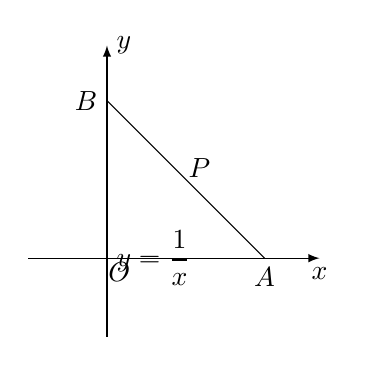
\begin{tikzpicture}
	\draw[domain=0.4:2.5,smooth,samples=100]  plot[id=1] function{1/x} node[right] {$y=\dfrac{1}{x}$};
	\draw[-latex] (-1,0) -- ++ (3.7,0) node[below] {$x$};
	\draw[-latex] (0,-1) -- ++ (0,3.7) node[right] {$y$};
	\node[below=5pt,right=-3pt] at (0,0) {$O$};
	\draw (0,2) node[left] {$B$} -- node[right=5pt,above=-3pt] {$P$} (2,0) node[below] {$A$};
\end{tikzpicture}
\end{document}